\documentclass[parskip]{scrartcl}
%docummentclass{standalone}
\usepackage[margin=15mm]{geometry}
\usepackage{tikz}


\begin{document}

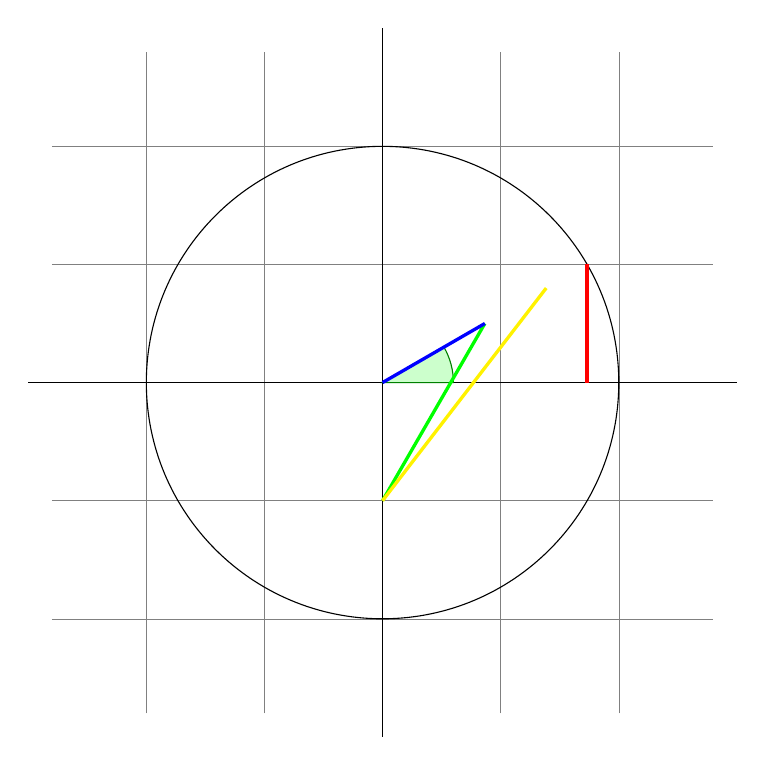
\begin{tikzpicture}[scale=3]
    %\clip (-0.1,-0.2) rectangle (1.1,0.75);
    \draw[step=.5cm,gray,very thin] (-1.4,-1.4) grid (1.4,1.4);
    \draw (-1.5,0) -- (1.5,0);
    \draw (0,-1.5) -- (0,1.5);
    \draw (0,0) circle [radius=1cm];
    \filldraw[fill=green!20,draw=green!50!black] (0,0) -- (3mm,0mm)
    arc [start angle=0, end angle=30, radius=3mm] -- cycle;
    %+(0,-0.5)
    % +means the endpoint is relative to the starting point (30:1cm)
    \draw[red,very thick] (30:1cm) -- +(0,-0.5);
    % (0,-1.5)
    % ++ means the endpoint is relative to the starting point (30:0.5cm)
    % (0, -1.5cm) means the line extends 0 unit in x direction and -1.5 unit in the y direction
    % current position moves to the end of the line
    %\draw[black,very thick] (30:1cm) -- ++(0,-0.5);
    \draw[green,very thick] (30:0.5cm) -- (0,-0.5);
    \draw[yellow,very thick] (30:0.8cm) -- (0,-0.5);
    \draw[blue,very thick] (0.433cm, 0.25cm) -- (0,0);

\end{tikzpicture}

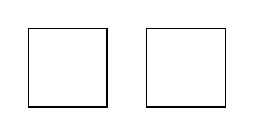
\begin{tikzpicture}
    \def\rectanglepath{-- ++(1cm,0cm) -- ++(0cm,1cm) -- ++(-1cm,0cm) -- cycle}
    \draw (0,0) \rectanglepath;
    \draw (1.5,0) \rectanglepath;
\end{tikzpicture}

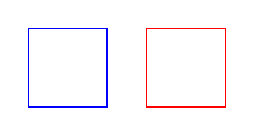
\begin{tikzpicture}
    \def\rectanglepath{-- +(1cm,0cm) -- +(1cm,1cm) -- +(0cm,1cm) -- cycle}
    \draw[blue] (0,0) \rectanglepath;
    \draw[red] (1.5,0) \rectanglepath;
\end{tikzpicture}


\end{document}